\chapter{Desarrollo Experimental y Resultados}

\section{Experimento 1: Medición de Inductancia mediante Onda de Corriente Triangular}

\subsection{Esquema y Principio de Funcionamiento}
Para aproximar un generador de corriente ideal a partir de un generador de funciones con tensión de salida $V$, se
conecta en serie un resistor $r = 100\kohm$, cuyo valor es mayor que la impedancia de la bobina con núcleo magnético
ensayada ($r \gg |Z_L|$). El esquema del circuito y el montaje de laboratorio se muestran en la Figura
\ref{fig.ej1:circuito_y_montaje}.

\begin{figure}[!ht]
    \centering
    \begin{subfigure}[c]{0.48\textwidth}
        \centering
        \begin{circuitikz}[scale=0.75]
    \draw (0,0) to[sV, l={$V_{\text{gen}}$}] (0,3)
          to[R, l={$r = 100\kohm$}] (3,3)
          to[R, l={$R$}] (3,1.5)
          to[L, l={$L$}] (3,0)
          to[short] (0,0);
    \draw (3,3) to[short, *-o] (4.5,3) node[right] {\small CH2(+)};
    \draw (3,0) to[short, *-o] (4.5,0) node[right] {\small GND};
    \draw (0,3) to[short, *-o] (-1.5,3) node[left] {\small CH1(+)};
\end{circuitikz}

        \caption{Esquema del circuito de medición.}
        \label{crkt.ej1:esquema}
    \end{subfigure}
    \hfill
    \begin{subfigure}[c]{0.48\textwidth}
        \centering
        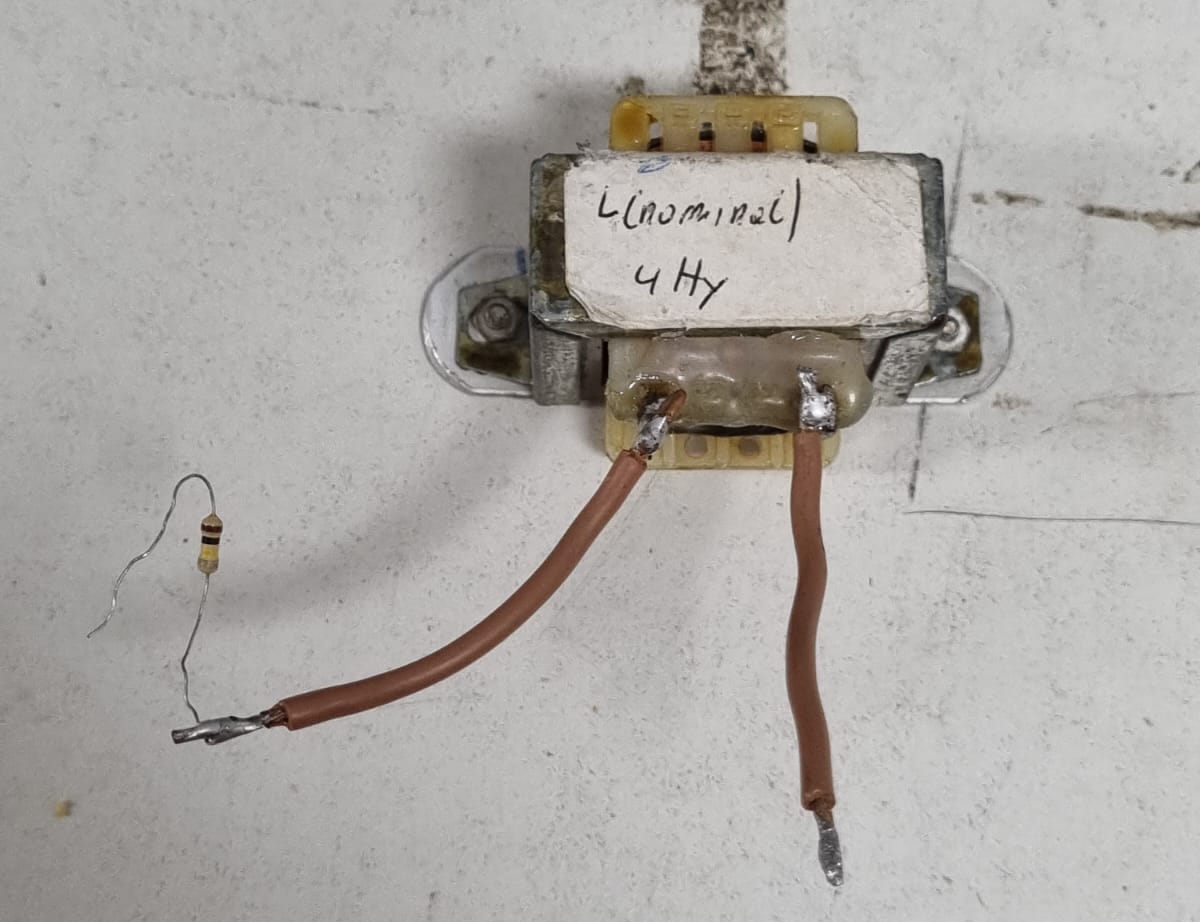
\includegraphics[width=\textwidth]{pictures/crkt_ind.jpeg}
        \caption{Montaje experimental en el pañol.}
        \label{fig.ej1:montaje}
    \end{subfigure}
    \caption{Circuito de medición y montaje del ensayo con corriente triangular.}
    \label{fig.ej1:circuito_y_montaje}
\end{figure}

La tensión observada en el Canal 2 sobre el inductor es la superposición de la componente inductiva pura $v_L(t)$ y la
caída resistiva $v_R(t)$, produciendo una forma de onda compuesta $v(t) = v_L(t) + v_R(t)$. La componente reactiva
$v_L(t)$ genera un escalón rectangular de tensión cuya amplitud pico a pico es $V_{pp} = 2 \cdot V_L$, mientras que la
componente resistiva $v_R(t)$ sigue la pendiente de rampa de la corriente, midiéndose su amplitud como $V_R$.

En la Figura \ref{fig.ej1:ondas_esperadas} se representan las formas de onda teóricas esperadas y se señalan los rangos de
tensión de los cuales se extraen las magnitudes medidas $V_{pp}$ y $V_R$.

\begin{figure}[!ht]
    \centering
    \begin{tikzpicture}[scale=0.9, >=stealth]
    % --- 1. Corriente i(t) ---
    \draw[->] (-0.8, 4.5) -- (9.0, 4.5) node[right] {$t$};
    \draw[->] (0, 3.0) -- (0, 6.2) node[above left] {$i(t)$};
    \draw[thick, blue] (0,4.5) -- (2,5.7) -- (4,3.3) -- (6,5.7) -- (8,3.3);
    
    \draw[dashed, gray] (2,4.5) -- (2,5.7);
    \draw[<->] (2.3, 4.5) -- (2.3, 5.7) node[midway, right, fill=white, inner sep=1pt] {$I$};

    % --- 2. Tensión inductiva pura v_L(t) ---
    \draw[->] (-0.8, 1.2) -- (9.0, 1.2) node[right] {$t$};
    \draw[->] (0, -0.2) -- (0, 2.7) node[above left] {$v_L(t) = L \frac{di}{dt}$};
    \draw[thick, red] (0,2.1) -- (2,2.1) -- (2,0.3) -- (4,0.3) -- (4,2.1) -- (6,2.1) -- (6,0.3) -- (8,0.3);
    
    \draw[<->] (6.5, 0.3) -- (6.5, 2.1) node[midway, right, fill=white, inner sep=1pt] {$V_{pp} = 2 e_L$};

    % --- 3. Tensión total compuesta v(t) = v_L(t) + v_R(t) ---
    \draw[->] (-0.8, -2.5) -- (9.0, -2.5) node[right] {$t$};
    \draw[->] (0, -4.3) -- (0, -0.7) node[above left] {$v(t) = v_L(t) + v_R(t)$};
    \draw[thick, purple] (0,-1.7) -- (2,-1.1) -- (2,-3.3) -- (4,-2.7) -- (4,-1.7) -- (6,-1.1) -- (6,-3.3) -- (8,-2.7);

    % Cotas de extraccion de tensiones compuestas
    % Rampa resistiva V_R
    \draw[dashed, gray] (2,-1.1) -- (3.6,-1.1);
    \draw[dashed, gray] (2,-1.7) -- (3.6,-1.7);
    \draw[<->] (3.3, -1.7) -- (3.3, -1.1) node[midway, right, fill=white, inner sep=1pt] {$V_R = I \cdot R$};

    % Escalón inductivo pico a pico V_pp
    \draw[dashed, gray] (2,-1.7) -- (0.8,-1.7);
    \draw[dashed, gray] (2,-3.3) -- (0.8,-3.3);
    \draw[<->] (1.1, -3.3) -- (1.1, -1.7) node[midway, right, fill=white, inner sep=1pt] {$V_{pp} = 2 e_L$};
\end{tikzpicture}

    \caption{Formas de onda esperadas.}
    \label{fig.ej1:ondas_esperadas}
\end{figure}

La corriente eficaz/pico $I$ que circula por el circuito se calcula descontando las caídas de tensión en la bobina del
valor total producido por el generador:
\begin{equation}
    I = \frac{V - (V_R + V_{pp})}{r}
    \label{eq.ej1:calculo_corriente}
\end{equation}

\subsection{Mediciones y Cálculos}
Se varió la frecuencia de la señal triangular en $f = 50\Hz$, $100\Hz$ y $200\Hz$. Los resultados obtenidos y los
valores calculados para la inductancia $L$ y la resistencia serie $R$ se presentan en la Tabla \ref{tab.ej1:mediciones}.

\begin{table}[!ht]
    \centering
    \begin{tabular}{|c|c|c|c|}
        \hline
        \textbf{Frecuencia ($f$)} & \textbf{50 Hz} & \textbf{100 Hz} & \textbf{200 Hz} \\ \hline
        Resistencia serie $r$ ($\kohm$) & 100 & 100 & 100 \\ \hline
        Tensión de entrada $V$ ($\V$) & 10.1 & 10.2 & 10.2 \\ \hline
        Tensión pico a pico $V_{pp} = 2 \cdot V_L$ ($\mV$) & 87.2 & 170.0 & 340.0 \\ \hline
        Tensión resistiva $V_R$ ($\mV$) & 20.8 & 26.0 & 52.0 \\ \hline
        Corriente calculada $I$ ($\uA$) & 99.90 & 100.04 & 98.08 \\ \hline
        \textbf{Inductancia $L$ ($\text{H}$)} & \textbf{4.36} & \textbf{4.25} & \textbf{4.33} \\ \hline
        \textbf{Resistencia $R$ ($\Omega$)} & \textbf{208.20} & \textbf{259.84} & \textbf{530.12} \\ \hline
    \end{tabular}
    \caption{Resultados medidos y calculados para la bobina con núcleo magnético.}
    \label{tab.ej1:mediciones}
\end{table}

\subsection{Resultado Definitivo y Análisis}
Tomando la mediana de los valores de inductancia obtenidos a las tres frecuencias de ensayo:
\begin{equation}
    L_{\text{medido}} = \text{mediana}(4.36\text{ H}, 4.25\text{ H}, 4.33\text{ H}) = 4.33\text{ H}
    \label{eq.ej1:mediana_L}
\end{equation}

Se observa que mientras la inductancia $L$ se mantiene prácticamente constante, la resistencia serie de pérdidas $R$
aumenta significativamente con la frecuencia. Este marcado incremento es característico de las bobinas con núcleo
magnético de hierro. A baja frecuencia, la resistencia corresponde mayormente al bobinado de cobre. Al elevar
la frecuencia, las pérdidas por corrientes parásitas de Foucault inducidas en las chapas del núcleo ($P_e \propto f^2$)
y las pérdidas por histéresis magnética ($P_h \propto f$) aumentan considerablemente, provocando un aumento en la resistencia
equivalente de pérdidas.

\subsection{Formas de Onda Capturadas}
En las figuras \ref{fig.ej1:file0}, \ref{fig.ej1:file1} y \ref{fig.ej1:file2} se muestran las capturas obtenidas
en el osciloscopio para cada frecuencia.

\begin{figure}[!ht]
    \centering
    \begin{subfigure}[t]{0.45\textwidth}
        \centering
        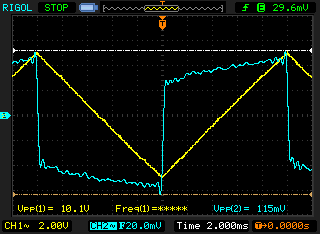
\includegraphics[width=\textwidth]{images/NewFile0.png}
        \caption{$f = 50\Hz$.}
        \label{fig.ej1:file0}
    \end{subfigure}
    \hfill
    \begin{subfigure}[t]{0.45\textwidth}
        \centering
        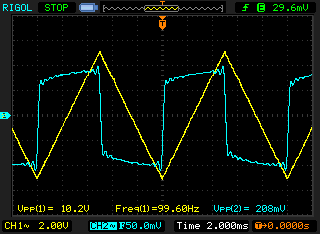
\includegraphics[width=\textwidth]{images/NewFile1.png}
        \caption{$f = 100\Hz$.}
        \label{fig.ej1:file1}
    \end{subfigure}
    \vspace{0.3cm}
    \begin{subfigure}[t]{0.45\textwidth}
        \centering
        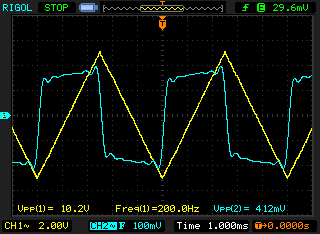
\includegraphics[width=\textwidth]{images/NewFile2.png}
        \caption{$f = 200\Hz$.}
        \label{fig.ej1:file2}
    \end{subfigure}
    \caption{Formas de onda en el osciloscopio: CH1 (amarillo, $V_{\text{gen}}$) y CH2 (cian, $V_L$).}
    \label{fig.ej1:oscilogramas}
\end{figure}

\section{Experimento 2: Medición de RSE en Capacitores Electrolíticos}

\subsection{Esquema y Principio de Funcionamiento}
Para medir la RSE de capacitores electrolíticos, se aplica una corriente de forma de onda cuadrada utilizando el
generador de funciones y una resistencia serie $r = 1\kohm$. El esquema del circuito y el montaje de laboratorio se
ilustran en la Figura \ref{fig.ej2:circuito_y_montaje}.

\begin{figure}[!ht]
    \centering
    \begin{subfigure}[c]{0.48\textwidth}
        \centering
        \begin{circuitikz}[scale=0.75]
    \draw (0,0) to[sV, l={$V_{\text{gen}}$}] (0,3)
          to[R, l={$r = 1\kohm$}] (3,3)
          to[R, l={\text{RSE}}] (3,1.5)
          to[C, l={$C$}] (3,0)
          to[short] (0,0);
    \draw (3,3) to[short, *-o] (4.5,3) node[right] {\small CH2(+)};
    \draw (3,0) to[short, *-o] (4.5,0) node[right] {\small GND};
    \draw (0,3) to[short, *-o] (-1.5,3) node[left] {\small CH1(+)};
\end{circuitikz}

        \caption{Esquema del circuito de medición.}
        \label{crkt.ej2:esquema}
    \end{subfigure}
    \hfill
    \begin{subfigure}[c]{0.48\textwidth}
        \centering
        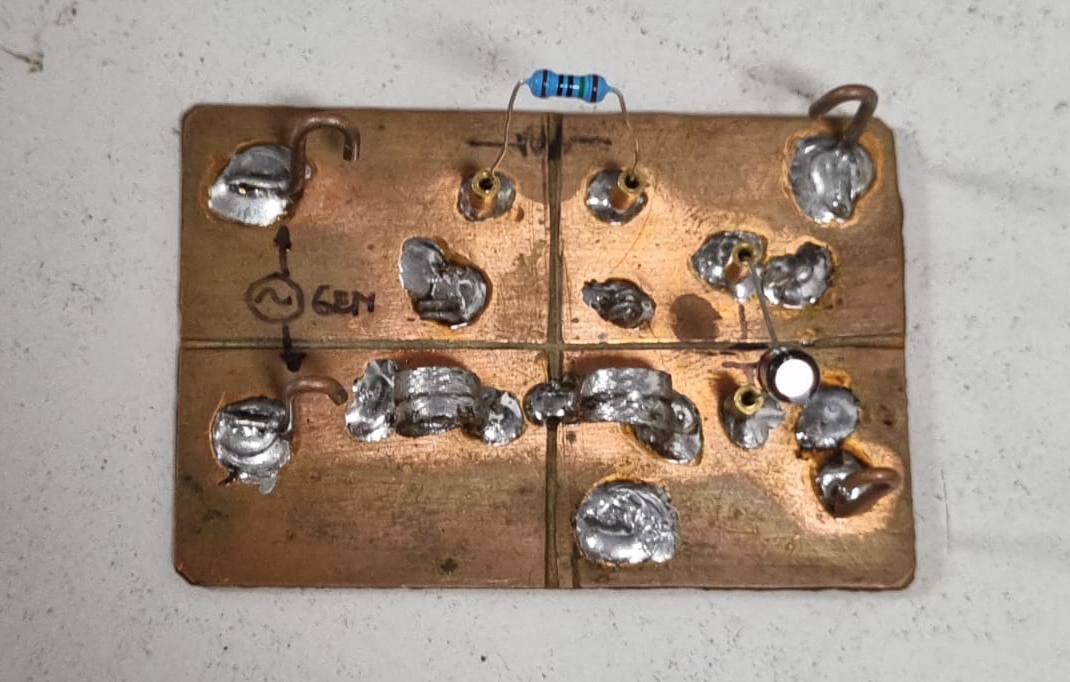
\includegraphics[width=\textwidth]{pictures/crkt_cap.jpeg}
        \caption{Montaje experimental en el pañol.}
        \label{fig.ej2:montaje}
    \end{subfigure}
    \caption{Circuito de medición y montaje del ensayo de RSE en capacitores.}
    \label{fig.ej2:circuito_y_montaje}
\end{figure}

La tensión en el capacitor real es la suma de la rampa de carga capacitiva $V_C$ y el salto resistivo instantáneo $e_R$
en los flancos de conmutación. En la Figura \ref{fig.ej2:ondas_esperadas} se representan las formas de onda teóricas
esperadas e indicación de los rangos de tensión de extracción.

\begin{figure}[!ht]
    \centering
    \begin{tikzpicture}[scale=0.9, >=stealth]
    % --- 1. Corriente cuadrada i(t) ---
    \draw[->] (-0.8, 4.5) -- (9.0, 4.5) node[right] {$t$};
    \draw[->] (0, 3.0) -- (0, 6.0) node[above left] {$i(t)$};
    \draw[thick, blue] (0,5.4) -- (2,5.4) -- (2,3.6) -- (4,3.6) -- (4,5.4) -- (6,5.4) -- (6,3.6) -- (8,3.6);

    % --- 2. Tensión compuesta v(t) = v_R(t) + v_C(t) ---
    \draw[->] (-0.8, 0.5) -- (9.0, 0.5) node[right] {$t$};
    \draw[->] (0, -2.0) -- (0, 2.8) node[above left] {$v(t) = v_{\text{RSE}}(t) + v_C(t)$};
    \draw[thick, purple] (0,0.5) -- (0,1.2) -- (2,2.1) -- (2,0.2) -- (4,-1.0) -- (4,0.7) -- (6,1.6) -- (6,-0.3) -- (8,-1.5);

    % Cotas de extracción de tensiones
    % Salto resistivo e_R
    \draw[dashed, gray] (2,2.1) -- (3.5,2.1);
    \draw[dashed, gray] (2,0.2) -- (3.5,0.2);
    \draw[<->] (3.1, 0.2) -- (3.1, 2.1) node[midway, right, fill=white, inner sep=1pt] {$e_R = I \cdot \text{RSE}$};

    % Rampa capacitiva V_C
    \draw[dashed, gray] (0,1.2) -- (1.5,1.2);
    \draw[dashed, gray] (2,2.1) -- (1.5,2.1);
    \draw[<->] (1.1, 1.2) -- (1.1, 2.1) node[midway, left, fill=white, inner sep=1pt] {$V_C$};
\end{tikzpicture}

    \caption{Formas de onda esperadas.}
    \label{fig.ej2:ondas_esperadas}
\end{figure}

La corriente producida por la onda cuadrada es $I = \frac{V}{r} = \frac{10.2\V}{1\kohm} = 10.2\mA$. El salto de
tensión brusco $e_R = V_R$ observado en los flancos de conmutación (como se aprecia en las figuras
\ref{fig.ej2:file3}, \ref{fig.ej2:file4} y \ref{fig.ej2:file5}) se debe exclusivamente a la RSE, mientras que la rampa
continua $V_C$ corresponde a la carga/descarga de la capacidad ideal $C$.

\subsection{Mediciones y Resultados}
La frecuencia de ensayo se fijó en $f = 10\si{\kilo\hertz}$ para tres capacitores de aluminio. Los datos medidos y los
valores de RSE calculados se consignan en la Tabla \ref{tab.ej2:mediciones}.

\begin{table}[!ht]
    \centering
    \begin{tabular}{|c|c|c|c|}
        \hline
        \textbf{Frecuencia ($f$)} & \textbf{10 kHz} & \textbf{10 kHz} & \textbf{10 kHz} \\ \hline
        Capacidad Nominal ($C$) & $1\uF$ & $2.2\uF$ & $4.7\uF$ \\ \hline
        Resistencia serie $r$ ($\kohm$) & 1 & 1 & 1 \\ \hline
        Tensión en capacitor $V_C$ ($\mV$) & 300 & 180 & 98.4 \\ \hline
        Corriente calculada $I = V/r$ ($\mA$) & 10.2 & 10.2 & 10.2 \\ \hline
        Tensión de salto resistivo $V_R = e_R$ ($\mV$) & 30.0 & 38.0 & 24.8 \\ \hline
        \textbf{RSE $= e_R / I$ ($\Omega$)} & \textbf{2.94} & \textbf{3.72} & \textbf{2.43} \\ \hline
    \end{tabular}
    \caption{Valores medidos y RSE calculada para capacitores electrolíticos.}
    \label{tab.ej2:mediciones}
\end{table}

\subsection{Formas de Onda Capturadas}
En las figuras \ref{fig.ej2:file3}, \ref{fig.ej2:file4} y \ref{fig.ej2:file5} se observan los saltos
de tensión instantáneos $e_R = V_R$ en los flancos de conmutación producidos por la RSE en el osciloscopio.

\begin{figure}[!ht]
    \centering
    \begin{subfigure}[t]{0.46\textwidth}
        \centering
        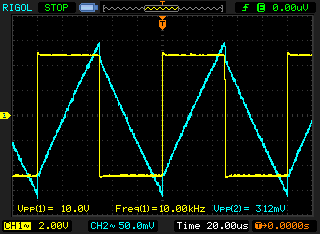
\includegraphics[width=\textwidth]{images/NewFile3.png}
        \caption{$C = 1\uF$.}
        \label{fig.ej2:file3}
    \end{subfigure}
    \hfill
    \begin{subfigure}[t]{0.46\textwidth}
        \centering
        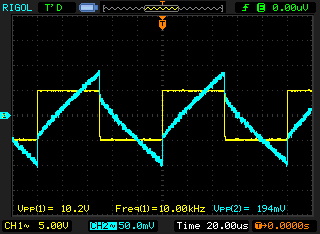
\includegraphics[width=\textwidth]{images/NewFile4.png}
        \caption{$C = 2.2\uF$.}
        \label{fig.ej2:file4}
    \end{subfigure}
    \vspace{0.3cm}
    \begin{subfigure}[t]{0.46\textwidth}
        \centering
        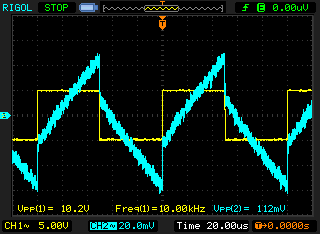
\includegraphics[width=\textwidth]{images/NewFile5.png}
        \caption{$C = 4.7\uF$.}
        \label{fig.ej2:file5}
    \end{subfigure}
    \caption{Formas de onda en osciloscopio: CH1 ($V_{\text{gen}}$) y CH2 (tensión total en $C$).}
    \label{fig.ej2:oscilogramas}
\end{figure}

\section{Experimento 3: Medición de Inductancia por el Método de Resonancia}

\subsection{Esquema y Principio de Funcionamiento}
Se conectó la bobina con núcleo de aire en serie con un capacitor conocido ($C_{\text{nom}} = 10\nF$) y un resistor
de protección $r = 50\ohm$. Se excitó la rama LC serie con una onda senoidal de frecuencia variable hasta detectar
la condición de resonancia. El esquema del circuito y el montaje de laboratorio se muestran en la Figura
\ref{fig.ej3:circuito_y_montaje}.

\begin{figure}[!ht]
    \centering
    \begin{subfigure}[c]{0.48\textwidth}
        \centering
        \begin{circuitikz}[scale=0.85]
    \draw (0,0) to[sV, l={$V_{\text{gen}}$}] (0,4.2)
          to[R, l={$r = 50\ohm$}] (3.5,4.2)
          to[R, l={$R$}] (3.5,2.8)
          to[L, l={$L$}] (3.5,1.4)
          to[C, l={$C$}] (3.5,0)
          to[short] (0,0);
    \draw (3.5,1.4) to[short, *-o] (4.8,1.4) node[right] {\small CH1 ($e_C$)};
    \draw (3.5,4.2) to[short, *-o] (4.8,4.2) node[right] {\small CH2 ($e_{\text{total}}$)};
    \draw (3.5,0) to[short, *-o] (4.8,0) node[right] {\small GND};
\end{circuitikz}

        \caption{Esquema del circuito resonante.}
        \label{crkt.ej3:esquema}
    \end{subfigure}
    \hfill
    \begin{subfigure}[c]{0.48\textwidth}
        \centering
        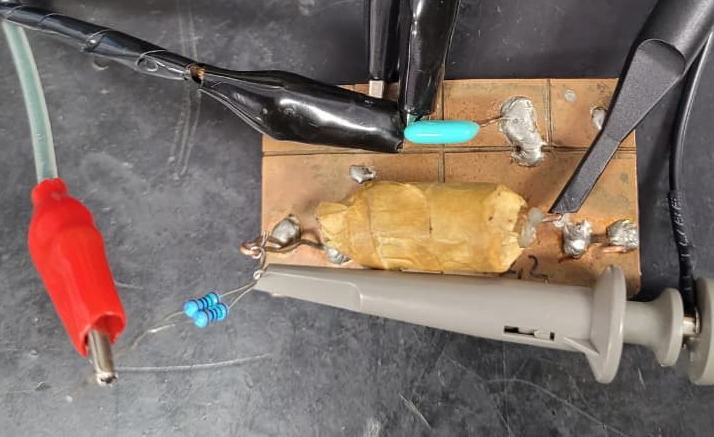
\includegraphics[width=\textwidth]{pictures/crkt_rc.jpeg}
        \caption{Montaje experimental en el pañol.}
        \label{fig.ej3:montaje}
    \end{subfigure}
    \caption{Circuito resonante LC serie y montaje del ensayo.}
    \label{fig.ej3:circuito_y_montaje}
\end{figure}

En resonancia ($f_0$), la reactancia inductiva anula a la reactancia capacitiva ($X_L = X_C$), de modo que la tensión
en el capacitor alcanza su máximo valor relativo $e_C$.

\subsection{Mediciones, Cálculo de Inductancia y Factor de Mérito}
Varíando la frecuencia del generador de funciones, se determinó experimentalmente la frecuencia de resonancia
$f_0 = 11.79\si{\kilo\hertz}$ al observar el pico máximo de tensión en el capacitor ($e_C = 660\mV$). Con el capacitor
nominal de prueba $C = 10\nF$, la inductancia de la bobina con núcleo de aire se calcula mediante la fórmula de Thomson:
\begin{equation}
    L = \frac{1}{(2 \pi f_0)^2 \cdot C} = \frac{1}{(2 \pi \cdot 11.79\si{\kilo\hertz})^2 \cdot 10\nF} \approx 18.2\mH
    \label{eq.ej3:calculo_L}
\end{equation}

Asimismo, se buscaron las frecuencias de corte superior ($f_1$) e inferior ($f_2$) donde la tensión en el capacitor cae al
$70,7\%$ del valor máximo ($0.707 \cdot e_{C\max}$). Los resultados se resumen en la Tabla \ref{tab.ej3:mediciones}.

\begin{table}[!ht]
    \centering
    \begin{tabular}{|l|c|c|c|c|}
        \hline
        \textbf{Condición} & \textbf{Frecuencia ($f$)} & \textbf{$e_C$ (CH2)} & \textbf{$e_{\text{total}}$ (CH1)} & \textbf{$Q = e_C / e_{\text{total}}$} \\ \hline
        $f_1$ (Corte Superior) & $17.99\si{\kilo\hertz}$ & $464\mV$ & $2.56\V$ & 0.1812 \\ \hline
        \textbf{$f_0$ (Resonancia)} & \textbf{11.79 kHz} & \textbf{660 mV} & \textbf{3.64 V} & \textbf{0.1813} \\ \hline
        $f_2$ (Corte Inferior) & $2\si{\hertz}$ & $456\mV$ & $4.64\V$ & 0.0982 \\ \hline
    \end{tabular}
    \caption{Mediciones en resonancia y frecuencias de corte superior e inferior.}
    \label{tab.ej3:mediciones}
\end{table}

\subsection{Formas de Onda Capturadas}
Las figuras \ref{fig.ej3:file8}, \ref{fig.ej3:file7} y \ref{fig.ej3:file6} muestran las señales senoidales observadas en
el osciloscopio para cada frecuencia característica.

\begin{figure}[!ht]
    \centering
    \begin{subfigure}[t]{0.46\textwidth}
        \centering
        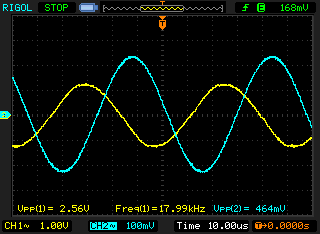
\includegraphics[width=\textwidth]{images/NewFile8.png}
        \caption{$f_1 = 17.99\si{\kilo\hertz}$ (frecuencia de corte superior).}
        \label{fig.ej3:file8}
    \end{subfigure}
    \hfill
    \begin{subfigure}[t]{0.46\textwidth}
        \centering
        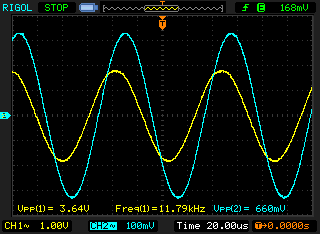
\includegraphics[width=\textwidth]{images/NewFile7.png}
        \caption{$f_0 = 11.79\si{\kilo\hertz}$ (frecuencia de resonancia).}
        \label{fig.ej3:file7}
    \end{subfigure}
    \vspace{0.3cm}
    \begin{subfigure}[t]{0.46\textwidth}
        \centering
        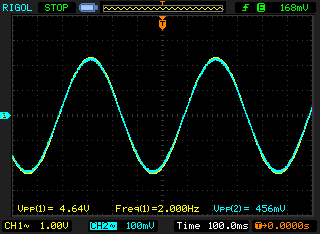
\includegraphics[width=\textwidth]{images/NewFile6.png}
        \caption{$f_2 = 2\si{\hertz}$ (frecuencia de corte inferior).}
        \label{fig.ej3:file6}
    \end{subfigure}
    \caption{Formas de onda senoidales en osciloscopio para el ensayo de resonancia.}
    \label{fig.ej3:oscilogramas}
\end{figure}
